\newcommand{\minipagespace}[1]{
	\begin{minipage}[c]{#1\textwidth}
		\ 
	\end{minipage}
}

\section{Culling}

Der erste Weg eine Voxel Engine zu optimieren wird
offensichtlich, wenn man sich einen Würfel aus $8$
Voxels betrachtet. Dabei beobachten wir, dass
die Hälfte der Seiten der Voxels nach innen schauen
und somit nicht sichtbar sind. Wenn man die
Seitenlänge dieses Würfels verdoppelt, multipliziert
man die Oberfläche mit $4$ und das Volumen mit $8$.
Somit entstehen immer mehr Seiten, die nach innen
schauen, umso größer das Objekt ist. Also wird
dies bei großen Objekten dazu führen, dass die
meisten Seiten nicht sichtbar sind.

\begin{center}
\begin{figure}[ht]
	\minipagespace{0.04}
	\begin{minipage}[c]{0.4\textwidth}
		\begin{center}
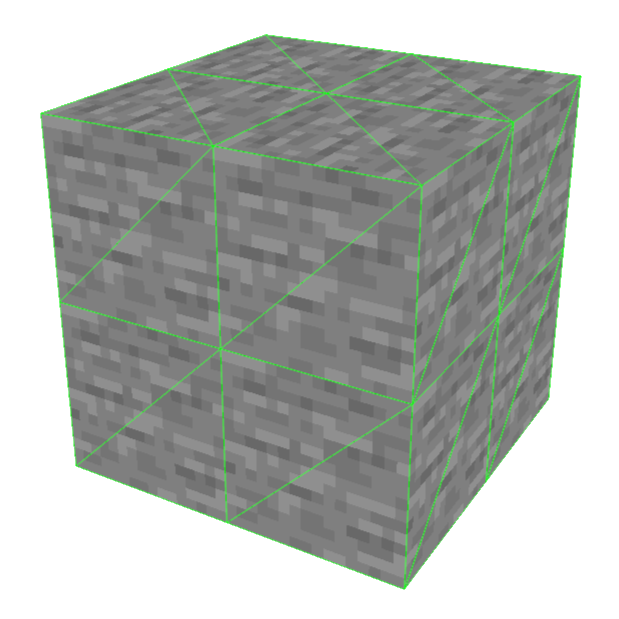
\includegraphics[width=1\textwidth]{../assets/culling/opaque_8_blocks.png}
		\end{center}
	\end{minipage}
	\minipagespace{0.09}
	\begin{minipage}[c]{0.4\textwidth}
		\begin{center}
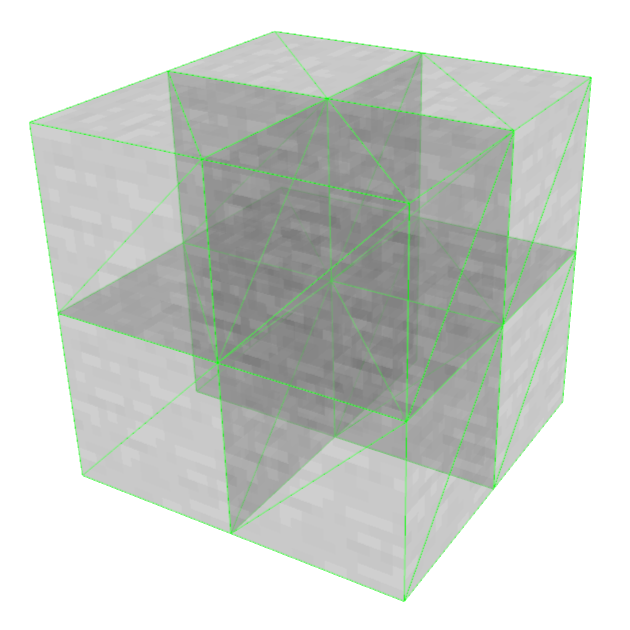
\includegraphics[width=1\textwidth]{../assets/culling/transparent_8_blocks.png}
		\end{center}
	\end{minipage}\hfill
\end{figure}
\end{center}

Mit \gqq{Culling} beschreibt man die Optimierung,
diese Seiten zu entfernen.

{ \subsection{Erste Implementation}

% TODO
 }

{ \subsection{Binäres Greedy Meshing}

Ich habe erst geplant, eine einfachere Implementation
von Greedy Meshing zu erstellen, bevor ich dies mit
einem binären Algorithmus mache, aber dadurch,
dass das Culling schon binär ist, ist die binäre
Greedy Meshing Implementation sogar einfacher als
eine andere.

Der Grundgedanke in dieser Implementation ist,
dass jedes Mal, wenn wir eine Seite betrachten,
wir versuchen diese erst in eine Richtung so weit
zu erweitern, bis keine Seite mehr da ist und dann
erweitern wir diesen ganzen Streifen in die andere
Richtung.
Während man das macht, entfernt man immer die
Bits in der Bitmaske, die gerade für diese Dreiecke
verwendet werden, damit sie nicht später für andere
Dreiecke wieder verwendet werden.

\begin{center}
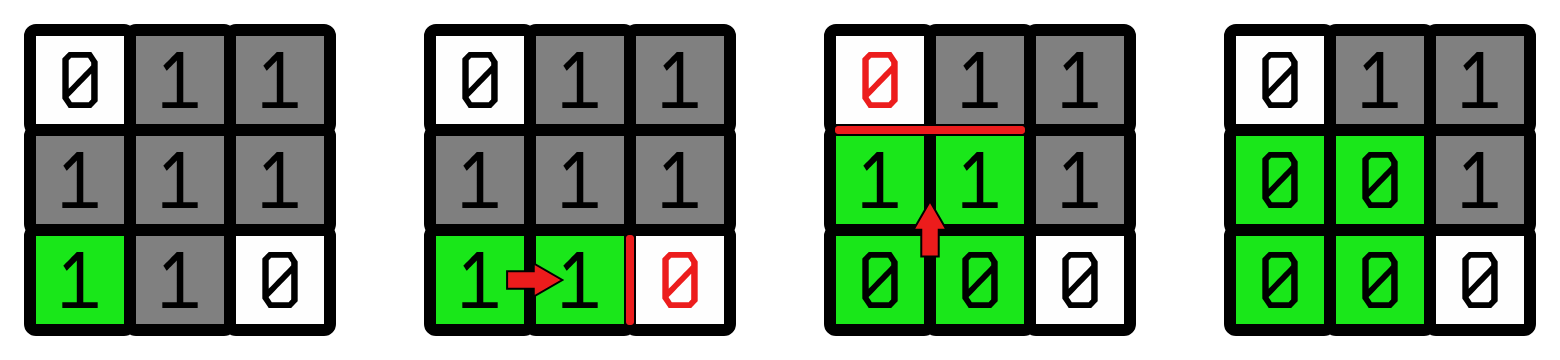
\includegraphics[width=0.95\textwidth]{../assets/greedy/grid_visualization.png}
\end{center}

Wenn wir eine Bitmaske haben, in der ein
32-Bit Integer eine Reihe von Seiten darstellt,
dann geht es sehr schnell, die Streifen zu erkennen,
da man mit den x86-Befehlen
\href{https://www.felixcloutier.com/x86/bsf}{BSF} \cite{bsf}
und
\href{https://www.felixcloutier.com/x86/bsr}{BSR} \cite{bsr}
die Anzahl von Nullen oder Einsen am Anfang oder
Ende eines 32-Bit Integers mit einem einzigen
Befehl berechnen kann.
Zudem kann man mit einem bitweisen ODER
überprüfen, ob der Streifen in die andere Richtung
erweitert werden kann, und man kann die Einträge
in der Bitmaske mit einem bitweisen UND entfernen.

\begin{lstlisting}[language=Rust]
let mut mask_copy = array[j];
let mut k = 0;
while mask_copy != 0 {
	let zeros = mask_copy.trailing_zeros();
	mask_copy >>= zeros;
	k += zeros;

	let ones = mask_copy.trailing_ones();
	mask_copy >>= ones;
	let from = k;
	k += ones;

	// Dieser gesamte Streifen als Bitmaske.
	// (Die wirkliche Implementation sieht etwas anders
	//  aus, da sich overflow von << komisch verhaelt)
	let strip_mask = ((1 << ones) - 1) << from;

	// Erweitere diesen Streifen in der Form eines Rechtecks
	// und entferne waehrenddessen 1en aus der Bitmaske.
	array[j] &= !strip_mask;
	let mut strip_expand = 0;
	for next_mask in &mut array[(j + 1)..] {
		if *next_mask & strip_mask == strip_mask {
			strip_expand += 1;
			*next_mask &= !strip_mask;
		} else {
			break;
		}
	}

	// erstelle ein Rechteck mit der richtigen Groesse...
}
\end{lstlisting}

Vielleicht ist Ihnen aber schon aufgefallen,
dass die Bitmaske, die wir für das Binäre Culling
verwendet haben, nicht in die richtige Richtung
ausgerichtet ist.
Dabei ist nämlich ein Integer eine Reihe von Voxels,
die sich gegenseitig verdecken können, während wir
hier eine Reihe von Voxels
(oder genauer: sichtbare Seiten)
brauchen, die nebeneinander liegen.
Deswegen müssen wir aus der Culling Bitmaske
eine neue Bitmaske konstruieren:

\begin{lstlisting}[language=Rust]
let culled_blocks_mask = // maske von Binaeres Culling
let mut greedy_mask = Box::<FaceMap<ChunkArray2D<u32>>>::default();
for (face, array2d) in culled_blocks_mask.iter_face() {
	for (i, array) in array2d.iter().enumerate() {
		for (j, mask) in array.iter().enumerate() {
			let mut mask = *mask;
			let mut k = 0;
			while mask != 0 {
				let zeros = mask.trailing_zeros();
				mask = (mask >> zeros) & !1;
				k += zeros;
				greedy_mask[face][k as usize][i] |= 1 << j;

				// Da horizontale Streifen von Voxels haeufiger
				// vorkommen als vertikale Streifen, mache ich,
				// dass die Bitmasken in den x- und z-Achsen
				// beide horizontal ausgerichtet sind.
				// Deswegen wird in der wirklichen Implementation
				// fuer die z-Achse `i` und `j` getauscht.
			}
		}
	}
}
greedy_mask
\end{lstlisting}

Wenn wir nun diese Bitmaske haben, können wir mit dem
oben genannten Algorithmus die Seiten zu größeren
Seiten kombinieren.
Wenn wir also diese Information benutzen,
um die Dreiecke größer zu machen, sind wir
schon mit dem Greedy Meshing fertig!

\vspace{0.5cm}

% Greedy Meshing 1 stats from: bench 11
\benchgraph{4}{0.25}{
	algo                   & blue       & red       \\
	Erste Implementation   & 12.834184  & 0.672563  \\
	Binäres Culling 1      &  2.883930  & 5.155590  \\
	Binäres Culling 2      &  8.524388  & 0.448866  \\
	Greedy Meshing 1       &  5.641821  & 0.425993  \\
}

Mit diesem Algorithmus erhalten wir sogar eine bessere
Performance, da wir weniger Dreiecke konstruieren
müssen.
Zudem ist die Anzahl von Dreiecken in einer
typischen Spielwelt jetzt von
1.857.984 Ecken und 928.992 Dreiecken
runter auf 809.484 Ecken und 404.742 Dreiecken
gesunken.
Somit haben wir etwa 2,3-mal weniger Dreiecke.

\vspace{0.7cm}

{
	\setlength{\parindent}{0pt}
	... eigentlich sind wir aber noch nicht ganz fertig!\\
	Wir haben noch ein Problem übersehen.
}
 }
